\documentclass{standalone}

\usepackage{ tikz }
\usepackage{ amssymb }
\usepackage{ amsmath }
\usepackage{ MnSymbol }
\usepackage{ stmaryrd }

\usetikzlibrary{shapes}

\begin{document}
    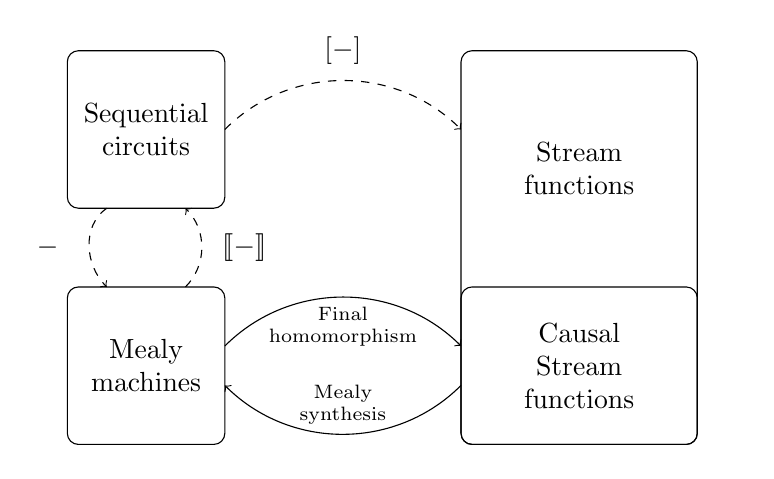
\begin{tikzpicture}
        \draw [rounded corners] (0,1) -- (1,1) -- (1,3) -- (-1,3) -- (-1,1) -- (0,1);
        \node [align=center] at (0,2) {Sequential \\ circuits};
        \coordinate (SC1) at (1,2); 
        \coordinate (SC2) at (-0.5, 1);
        \coordinate (SC3) at (0.5, 1);

        \draw [rounded corners] (0,0) -- (1,0) -- (1,-2) -- (-1,-2) -- (-1,0) -- (0,0);
        \node [align=center] at (0,-1) {Mealy\\ machines};

        \coordinate (MM1) at (-0.5,0);
        \coordinate (MM2) at (0.5, 0);
        \coordinate (MM3) at (1, -0.75);
        \coordinate (MM4) at (1, -1.25);

        \draw [rounded corners] (5,-2) -- (7,-2) -- (7,3) -- (4,3) -- (4,-2) -- (5,-2);
        \node [align=center] at (5.5,1.5) {Stream \\ functions};
        \coordinate (SF1) at (4,2); 

        \draw [rounded corners] (5,0) -- (7,0) -- (7,-2) -- (4,-2) -- (4,0) -- (5,0);
        \node [align=center] at (5.5,-1) {Causal \\ Stream \\ functions};
        \coordinate (CSF1) at (4,-0.75);
        \coordinate (CSF2) at (4,-1.25);

        \draw [->, dashed] (SC1) to[out=45,in=135] (SF1);
        \draw [->, dashed] (SC2) to[out=215, in=135] (MM1);
        \draw [->, dashed] (MM2) to[out=45, in=315] (SC3);

        \draw [->] (MM3) to[out=45,in=135] (CSF1);
        \draw [->] (CSF2) to[out=-135,in=-45] (MM4);

        \node at (2.5,3) {$[-]$};
        \node at (-1.25,0.5) {$\llangle-\rrangle$};
        \node at (1.25,0.5) {$\llbracket-\rrbracket$};
        \node [align=center, font=\scriptsize] at (2.5,-1.5) {Mealy \\ synthesis};
        \node [align=center, font=\scriptsize] at (2.5,-0.5) {Final \\ homomorphism};
        \node at (7.5,0) {};
    \end{tikzpicture}
\end{document}